\documentclass[12pt,letterpaper,noanswers]{exam}
\usepackage[usenames,dvipsnames,svgnames,table]{xcolor}
\usepackage[margin=0.9in]{geometry}
\renewcommand{\familydefault}{\sfdefault}
\usepackage{multicol}
\usepackage{wrapfig}
\pagestyle{head}
\header{AM 22b Class 37}{}{Apr 28: Differential equations, p.\thepage}
\runningheadrule
\headrule
\usepackage{graphicx} % more modern
\usepackage{amsmath} 
\usepackage{amssymb} 
\usepackage{hyperref}
\usepackage{tcolorbox}
\usepackage[utf8]{inputenc}
\usepackage{diagbox}
\usepackage{graphicx} 
\usepackage{enumitem}
\usepackage{tikz}
\tikzstyle{startstop} = [rectangle, rounded corners, minimum width=3cm, minimum height=1cm,text centered, draw=black]

\tikzstyle{process} = [rectangle, minimum width=3cm, minimum height=1cm, text centered, draw=black, fill=gray!20]
\tikzstyle{decision} = [ellipse, minimum width=3cm, minimum height=0.5cm, text centered, draw=black, fill=white!30]
\tikzstyle{arrow} = [thick,->,>=stealth]
\usetikzlibrary{shapes.geometric, arrows}
\pagenumbering{arabic}

\usepackage[numbered,autolinebreaks,useliterate]{mcode}

\newcommand{\mb}[1]{\underline{#1}}

\begin{document}
 \pdfpageheight 11in 
  \pdfpagewidth 8.5in




% I need to review the torus trajectories...

\begin{itemize}
% \item There is a pre-class assignment (20 minutes of videos + a few WeBWorK exercises) due at 10am this Monday.  It is available on Canvas.
\itemsep0em
\item PSet 10 is due Thurs Apr 29th at 6pm ET.
\item Our final skill check is today.
\item If it would be helpful for you to have an alternate deadline for PSet 10, make arrangements with me via direct message on Slack.
\item Quiz 07 (our final assignment) will be available from May 8th at 5pm to May 12th at 5pm.
\end{itemize}

\hrule
\vspace{0.2cm}

% partial derivatives, gradient
% local linearity, differential, directional deriv
% 2nd order partials + equations with partials

\noindent\textbf{Big picture}

We have approached ordinary differential equations from three perspectives: using approximate solutions (slope fields + Euler's method + RK45), finding exact solutions (rarely, using separation of variables), using qualitative methods (identifying equilibrium solutions and whether they are `stable' or `unstable').

Today we will introduce partial differential equations.

\vspace{0.2cm}
\hrule
\vspace{0.2cm}

\noindent\textbf{Teams}

\begin{multicols}{2}

1.  student names
\end{multicols}

\vspace{0.2cm}
\hrule
\vspace{0.2cm}

\noindent\textbf{Complex-valued eigenvalues}
\begin{tcolorbox}
\begin{itemize}
    \item \textbf{Euler's formula} says that $e^{ib} = \cos b + i\sin b$.
    \item Suppose $\underline{x}(t)$ is a complex valued solution to a linear system $\frac{d\underline{x}}{dt}= A\underline{x}$.  Suppose $\underline{x}(t) = \underline{x}_{\text{re}}(t) + i\underline{x}_{im}(t)$ where $\underline{x}_{\text{re}}(t)$ and $\underline{x}_{im}(t)$ are real-valued functions of $t$.  Then $\underline{x}_{re}(t)$ and $\underline{x}_{im}(t)$ are both solutions of the original system $\frac{d\underline{x}}{dt}= A\underline{x}$.
\end{itemize}
\emph{Theorem is from Blanchard, Devaney, and Hall, section 3.4: complex eigenvalues}

\end{tcolorbox}

Construct two real solutions to the system $\frac{d\underline{x}}{dt} = \left(\begin{array}{c c}-2 & -3 \\ 3 & -2\end{array}\right)\underline{x}$.

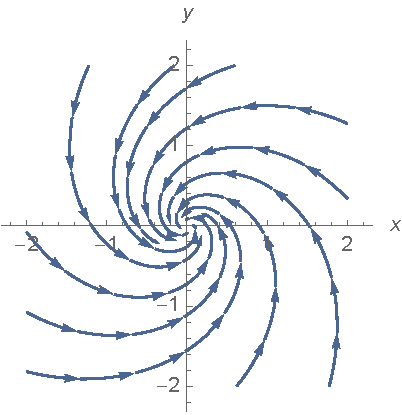
\includegraphics{img/C36phase.pdf}


\vspace{0.2cm}
\hrule
\vspace{0.2cm}


\noindent\textbf{Random walks: evolution in time AND space}
\begin{tcolorbox}
\begin{itemize}
\itemsep0em
    \item In a one-dimensional \textbf{random walk}, a walker starting at location $x_n$ at time $t_n$ has a probability $p$ of moving one unit left, to location $x_n - 1$, and a probability $1-p$ of moving one unit right, to location $x_n + 1$, at time $t_{n+1}$.
    \item A group of random walkers with $p=0.5$ who are all located at the origin at time $0$ have a distribution that evolves in space and in time.
    \item An ordinary differential equation can capture evolution in time, or evolution in space, but not both.  We can use a \textbf{partial differential equation} to describe the evolution of a function that depends on space and time.
\end{itemize}
\end{tcolorbox}
 

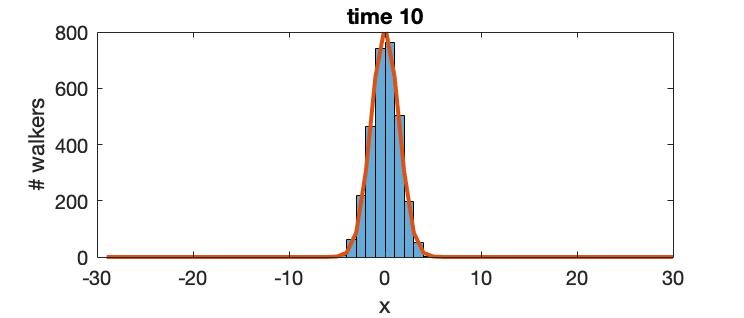
\includegraphics[width=0.45\linewidth]{img/C36p1a.png}
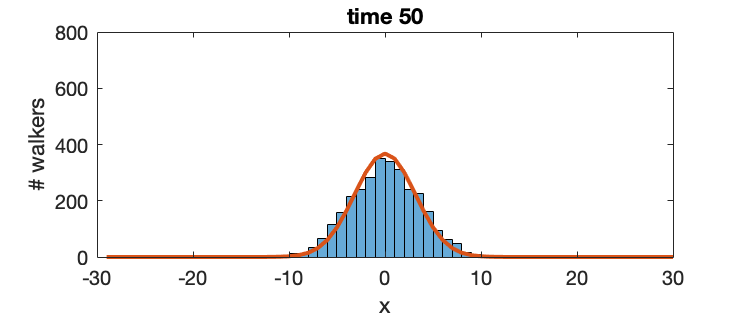
\includegraphics[width=0.45\linewidth]{img/C36p1b.png}


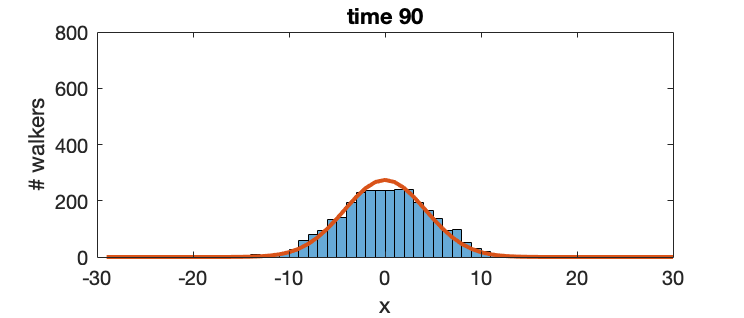
\includegraphics[width=0.45\linewidth]{img/C36p1c.png}
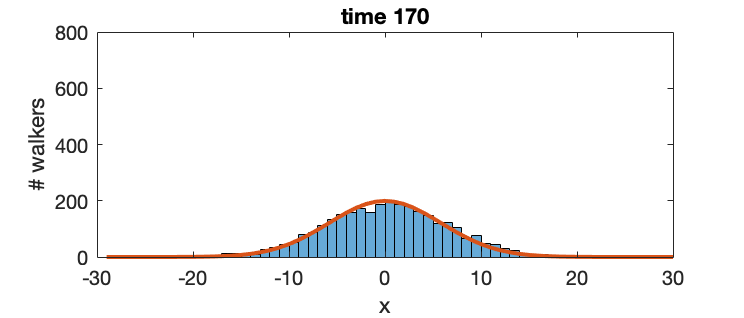
\includegraphics[width=0.45\linewidth]{img/C36p1d.png}

\vspace{0.2cm}
\hrule
\vspace{0.2cm}


\noindent\textbf{What is a pde?}
\begin{tcolorbox}
\begin{itemize}
\itemsep0em
    \item A \textbf{partial differential equation} is a differential equation with partial derivatives.  The presence of partial derivatives means that the dependent variable is a function of multiple independent variables.
    \item Just as for algebraic equations and for ordinary differential equations, it is worthwhile to distinguish between \textbf{linear} partial differential equations and nonlinear partial differential equations.
    \begin{itemize}
    \itemsep0em
        \item Linear example: $\partial_t u = c \partial_{xx} u$.
        \item Nonlinear example: $\partial_t u = u\partial_{xx} u$
    \end{itemize}
    \end{itemize}
\end{tcolorbox}
 \begin{tcolorbox}
\begin{itemize}
\itemsep0em   
    \item The \textbf{Laplace operator} or \textbf{Laplacian}, $\nabla^2 u = \partial_{xx} u + \partial_{yy} u$ (this is $\nabla^2 u = \nabla \cdot \nabla u$) often arises in partial differential equations.  It is sometimes written $\Delta u$.
    \item There are three prototypical types of linear PDEs:
    \begin{itemize}
    \itemsep0em
        \item \textbf{parabolic}: $y = x^2$ is an equation for a parabola.  $\partial_y u = \partial_{xx} u$ is an example of a parabolic pde.  $\partial_t u = D \partial_{xx} u$ is the \textbf{diffusion} equation.  The second derivative in space is associated with processes that have \textbf{spatial symmetry}.  A first derivative in space would be associated with processes that \textbf{are not symmetric}.
        \item \textbf{hyperbolic}: $x^2 - y^2 = 0$ is an equation for a hyperbola.  $\partial_{xx} u = \partial_{yy} u$ is an example of a hyperbolic pde.  $\partial_{tt} u = c^2 \partial_{xx}u$ is the \textbf{wave} equation.  
        \item \textbf{elliptic}: $x^2 + y^2 = 0$ is an equation for an ellipse.
        $\partial_{xx} u + \partial_{yy} u = 0$ is an example of an elliptic pde.  This is \textbf{Laplace's} equation.
    \end{itemize}
\end{itemize}
\end{tcolorbox}

\noindent\textbf{Example.  Verifying a solution}.  Consider the diffusion equation $\displaystyle u_t = u_{xx}$, with diffusion constant $D = 1$ (Note that $[D] = L^2/T$).  Show that the Gaussian function $\displaystyle u(x,t) = \dfrac{c}{\sqrt{t}}e^{-x^2/(4t)}$ satisfies this relationship.

\vspace{2.5in}

This time-evolving Gaussian has width $\sqrt{2t}$ (the distance from the origin grows as $\sqrt{t}$).  The evolution of the random walkers is well described by this function.  

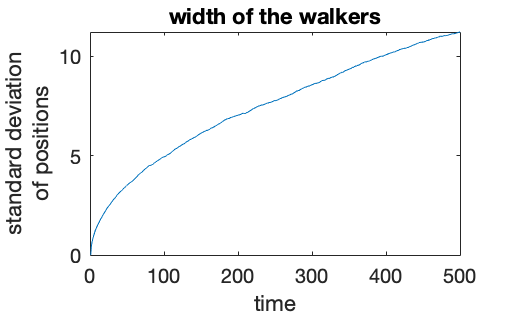
\includegraphics[width=0.5\linewidth]{img/C36p2.png}

    

\vspace{0.2cm}
\hrule
\vspace{0.2cm}

\eject

\noindent\textbf{Disciplined walkers}
\begin{tcolorbox}
\begin{itemize}
\itemsep0em
    \item Consider a group of `disciplined' walkers, whose distribution is given by $u(x,t)$.  Assume disciplined walkers always move to the right (or always move to the left), so that a walker at position $x_n$ in the $n$th timestep will be a position $x_n + a$ (or $x_n - a$), for a constant $a$, at the $n+1$st timestep.
\end{itemize}
\end{tcolorbox}
\noindent\textbf{Example.  Disciplined walker motion}.

Let $u(x,0)$ give the distribution of walkers at time $0$.  At time $\tau$, all the walkers have moved to the right by $a$ (so the walkers at $x=0$ move to $x=a$).  Write $u(x,a)$ in terms of $u(x,0)$.

\vspace{1in}

\noindent\textbf{Disciplined walker PDE.}

Consider the PDE $\partial_t f = -\frac{a}{\tau}\partial_x f$.  Use the chain rule to show that $f(x,t) = g\left(x - \frac{a}{\tau} t\right)$ satisfies the differential equation, with $f(x,0) = g(x)$.  \emph{Write $s = x - \frac{a}{\tau} t$.}

\vspace{2in}

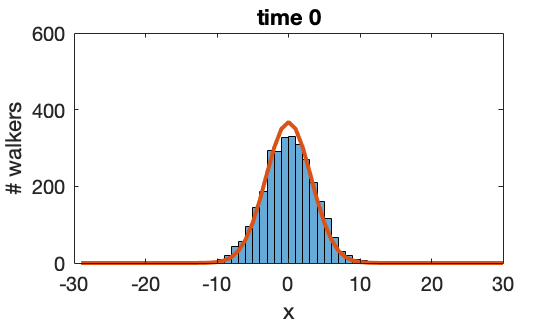
\includegraphics[width=0.24\linewidth]{img/C37p1a.png}
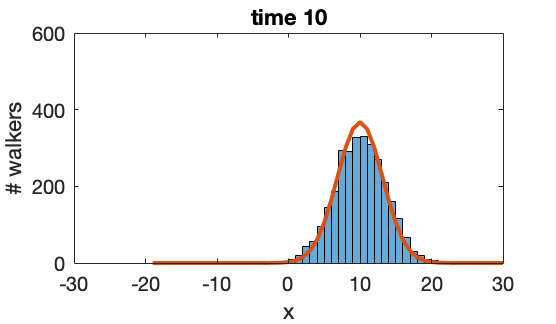
\includegraphics[width=0.24\linewidth]{img/C37p1b.png}
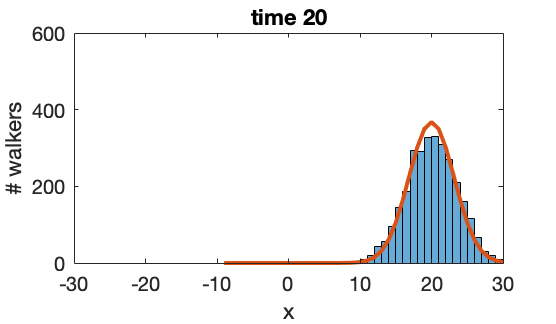
\includegraphics[width=0.24\linewidth]{img/C37p1c.png}
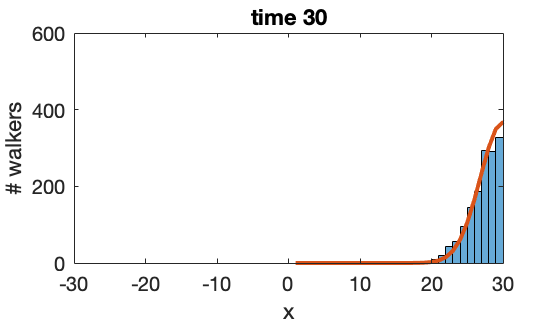
\includegraphics[width=0.24\linewidth]{img/C37p1d.png}

\vspace{0.2cm}
\hrule
\vspace{0.2cm}
\eject

% \noindent\textbf{Advection and diffusion}.
% \begin{tcolorbox}
% \begin{itemize}
% \itemsep0em
%     \item \textbf{Diffusion} is associated with (1) spread proportional to $\sqrt{t}$ (the distribution of random walkers spread out over time), (2) symmetry, (3) the rate of change depends on a second derivative in space.
%     \item \textbf{Advection} is associated with (1) transport (the distribution is shifted in one direction over time), (2) asymmetric motion, (3) the rate of change depends on a first derivative in space.
% \end{itemize}
% \end{tcolorbox}
% \noindent\textbf{Example.  Combining advection and diffusion}.

% Consider the pde $\partial_t u + c\partial_x u = \partial_{xx}u$.

% 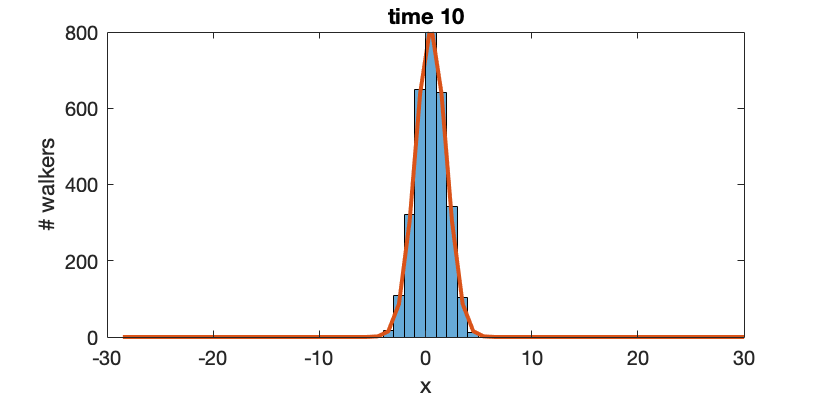
\includegraphics[width=0.24\linewidth]{img/C37p2a.png}
% 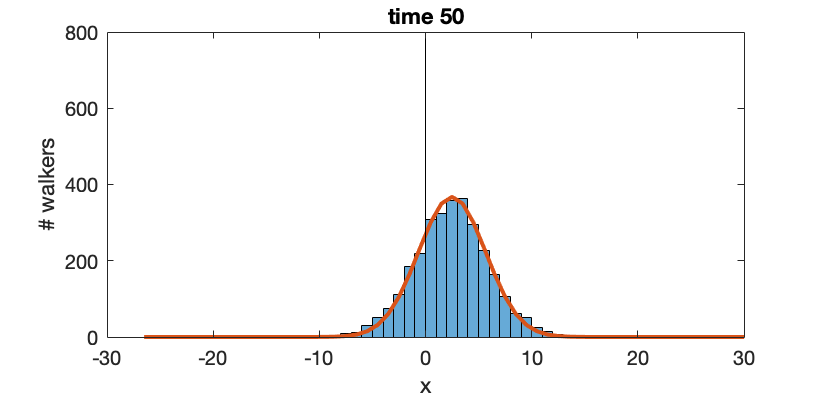
\includegraphics[width=0.24\linewidth]{img/C37p2b.png}
% 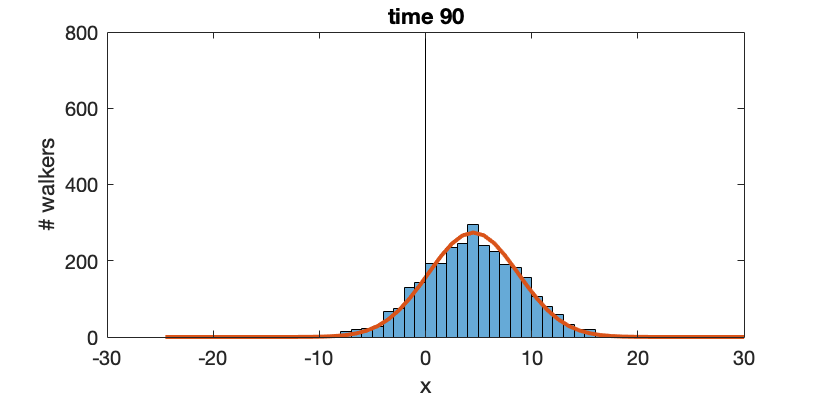
\includegraphics[width=0.24\linewidth]{img/C37p2c.png}
% 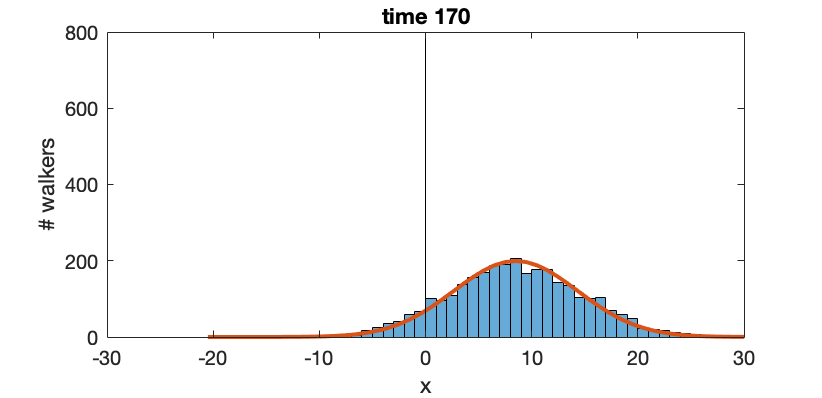
\includegraphics[width=0.24\linewidth]{img/C37p2d.png}

% We had $f(x,t) = \frac{k}{\sqrt{t}}e^{-x^2/(4t)}$ as a solution to $u_t = u_{xx}$.  We can use the chain rule to show that $f(x-ct,t)$ will satisfy the advection-diffusion equation above.

%  \emph{Write $s = x - c t$.  Find $\frac{\partial f}{\partial t}$ and $\frac{\partial f}{\partial t}$ in terms of $f_s$ and $f_t$}.

% % $\frac{\partial f}{\partial x} = f_s$, $\frac{\partial f}{\partial t} = f_s(-c) + f_t$

% % $\partial_t f + c\partial_x u = -cf_s + f_t + cf_s$

% \vspace{2.5in}

\vspace{0.2cm}
\hrule
\vspace{0.2cm}

\noindent\textbf{Where to go from here:}
\begin{tcolorbox}
\begin{itemize}
\itemsep0em
    \item complex analysis: line integrals and calculus in the complex plane (useful for signal processing and some types of data analysis).  apmth 104.
    \item approximate solution methods (and solution methods) for ODEs and PDEs.  apmth 105
    \item qualitative methods for analyzing ODEs (phase plane methods).  apmth 108
    \item using computers to approximate solutions to math problems.  apmth 111
    \item applications of linear algebra (with linear algebra review).  apmth 120
    \item optimization (a topic you encountered briefly in the fall).  apmth 121
    \item math modeling.  apmth 50 or apmth 115 (apmth 115 is recommended for juniors and seniors, and requires one of apmth 104/105/108 + stat 110 with some instructors)
\end{itemize}
\end{tcolorbox}

\end{document}